\subsection{Annahmen zur Modellierung}
Das Koordinatensystem des Flügels entspricht dem Flugzeugkoordinatensystem, sodass die Flügellängskoordinate durch y definiert ist. Der Koordinatenursprung ist im Lager A positioniert. \\

\noindent Der Holm inkl. des Holmstummels wird für die Belastung durch eine Prüfkraft $F_{pruef}$ in negative z-Richtung als Biegebalken ausgelegt. Dafür ist er an zwei Stellen gelagert, dem Lager $A$ und Lager $B$, dabei repräsentieren sie die Verstiftungen (siehe Bauteil "U-Profil"). Um eine Überbestimmung des Systems zu vermeiden, wird das Lager $B$ als Loslager angenommen. Die Querkraftbolzen werden nicht durch ein Lager, sondern durch eine zusätzlich angreifende Kraft $F_{Q}$ simuliert, da keine Absenkung, sondern lediglich eine Kraftaufnahme der Wurzelrippen möglich ist. \\

\noindent Als Randbedingungen der Modellierung sind die Halbspannweite $s$ und die Absenkung $w$ gegeben. Für die Absenkung $w$ soll eine Sicherheit $j=1,1$ gesetzt werden. Zwischen Lager $A$ und $B$ wird die Länge $l_{1}$ angenommen, zwischen Lager $B$ und der Wurzelrippe $C$ die Länge $l_{2}$. Die verbleibende Länge bis zur Flügelspitze, an der die Prüfkraft $F_{pruef}$ wirkt, wird $l_{3}$ bezeichnet. Die Halbspannweite $s$ wird beginnend in der Mitte der Verstiftungen bis zur Flügelspitze gemessen. Das Holmstummelende wird ab dem Lager $A$ mit $l_{0}$ als Länge definiert. Diese Länge ist jedoch unerheblich für die Modellierung, sondern wird erst für die Massenbestimmung benötigt.\\

\noindent Anhand der Randbedingungen und der Einspannvorrichtung für den Versuchsaufbau ergeben sich folgende Längen (ebenfalls in Abb. ~\ref{fig:Holmmodellierung}~ dargestellt): 
\begin{equation}
	s = 0,848 m
\end{equation}
\begin{equation}
	l_{0} = 0,03 m
\end{equation}
\begin{equation}
	l_{1} = 0,076 m
\end{equation}
\begin{equation}
	l_{2} = 0,037 m 
\end{equation}
\begin{equation}
	l_{3} = s - \frac{l_{1}}{2} - l_{2} = 0,773 m
\end{equation}
\begin{equation}
	w_{j=1,1} = \frac{1}{j} * w = \frac{1}{1,1} * 0,022 m = 0,02 m
\end{equation}
\begin{figure}
	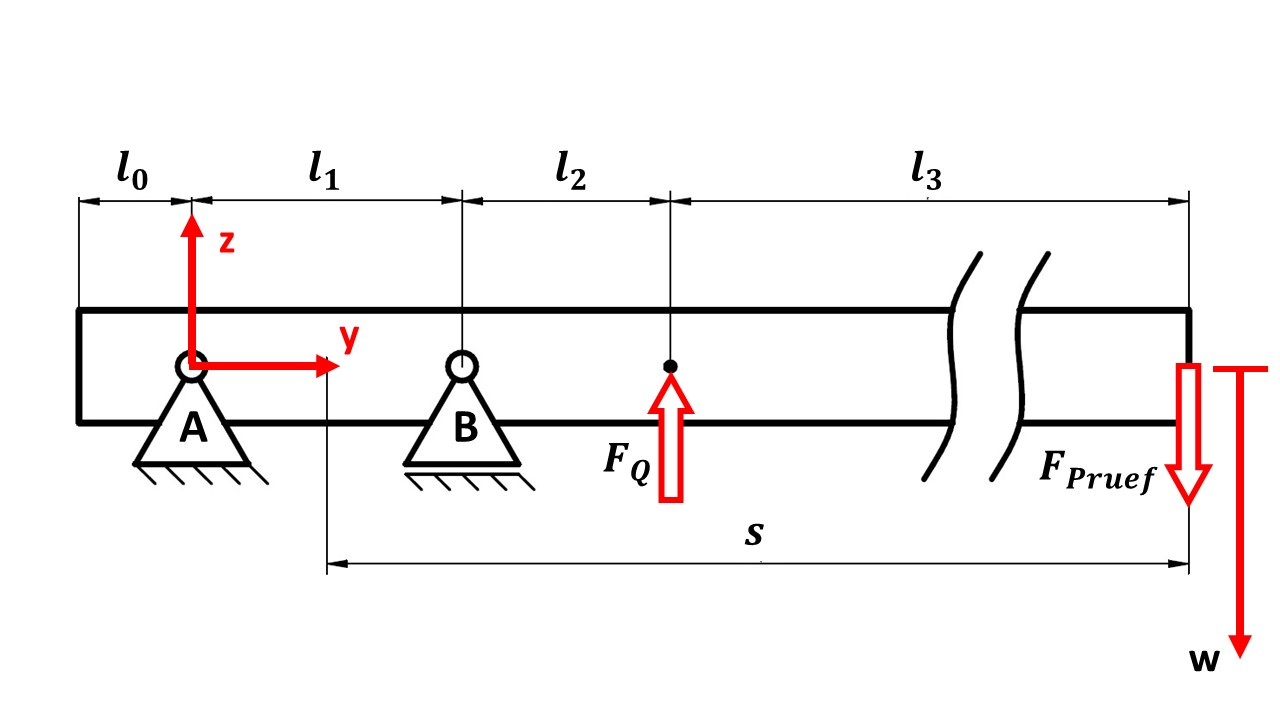
\includegraphics[width=1.0\textwidth]{Bilder/Balkenmodell.jpg}
	\caption{Modellierung des Holms}
	\label{fig:Holmmodellierung}
\end{figure}

\subsection{Analytische Lösung der Modellierung}



